\chapter{Pregled korištenih tehnologija}

\section{NFC \textit{(en. near-field communication)}}
NFC skup protokola omogućava uspostavu komunikacijskog kanala između dva uređaja koji se nalaze u neposrednoj blizini jedan drugog (1-4 cm) i razmjenu podataka između njih\cite{NFCProtocol}. Komunikacija se odvija na način da MASTER uređaj osluškuje signal na prijemniku i u slučaju detektovanje SLAVE signala uređaja pošiljaoca, propisanog istim standardom zaprima podatke i vrši obradu nad njima, komunikacija se u većini slučajeva odvija jednosmjerno kratkim standardiziranim porukama (NDEF), no moguće je ostvariti i half-duplex komunikaciju između uređaja, kao i razmjenu nestandardnih poruka, u kojem slučaju se sam korisnik mora pobrinuti za implementaciju kompletnog komunikacijskog protokola. Potpuni detalji implementacija dati su u referencama relevantnih standarda u nastavku tehničkog pregleda, odličnu sintezu detalja i implementacije daju Igoe, Coleman i Jepson\cite{Igoe2014}.
\subsection{NXP NTAG216}
U cilju zadovoljenja postavljenih funkcionalnih zahtjeva bilo je neophodno odabrati NFC Tag platformu koja će odrediti relevantne standarde pohrane binarnih podataka na uređajima kao i pripadajuće komunikacijske protokole, također dodatno su postavljeni zahtjevi ekonomičnosti implementacije i kompatibilnosti sa postojećim čitačima. Uzimajući u obzir nabrojane kriterije odabrana je platforma NTAG216 proizvođača NXP Semiconductors\cite{NTAG216} bazirana na NFC Forum Tag tipu 2 i ISO/IEC14443 Tip A specifikaciji\cite{NFCTag2}\cite{ISO14443}. 

\paragraph*{}
Mogućnosti navedene platforme dostatne su za ispunjenje navedenih funkcionalnih uslova, a pružaju i neke dodatne sigurnosne mehanizme - poput neizmjenjivog jedinstvenog serijskog broja svakog taga (Tag UID) potpisanog kriptografskim ključem proizvođača, navedena funkcionalnost nije implementirana u predstavljenom rješenju jer se bazira na zaštićenoj NXP tehnologiji i nije kompatibilna sa HCE emulacijom, no umnogome može doprinijeti ukupnoj sigurnosti fizičkih Tag čipova u slučaju produkcijske implementacije rješenja. U nastavku je data proizvođačka lista izdvojenih funkcionalnosti NTAG216:

\begin{itemize}[noitemsep]
    \item 7-bajtni UID programiran od strane proizvođača za svaki tag
    \item mogućnost jednokratnog programiranja i zaključavanja taga za dalje izmjene
    \item mogućnost read-only zaključavanja taga
    \item potpis originalnosti baziran na kriptografiji eliptičnih krivih
    \item zaštita memorijskih operacija 32-bitnom lozinkom
\end{itemize}

\paragraph*{}
Proces emulacije taga svodi se na što vjerniju reprezentaciju memorijskog prostora fizičkog uređaja u skadu sa relevantnim standardima, a opcionalno i dodatnih nestandardnih funkcionalnosti u vidu komunikacijskog protokola za korištenje naprednih funkcionalnosti date platforme. Kao minimum neophodan za standardnu komunikaciju NDEF porukama potrebno je emulirati generičko zaglavlje u obliku \textit{CC - capability container} i potpun zapis same NDEF poruke unutar korisničkog memorijskog prostora, potpun prikaz organizacije memorije NTAG216 platforme dat je na slici \ref{fig:ntag_mem}. Za emulaciju nestandardnih dijelova, poput zaštite čitanja korisničkog memorijskog prostora lozinkom ili emulaciju serijskog broja, za svaku različitu platformu neophodno je implementirati komunikacijski protokol u skladu sa proizvođačkom specifikacijom.

\begin{figure}[H]
    \centering
    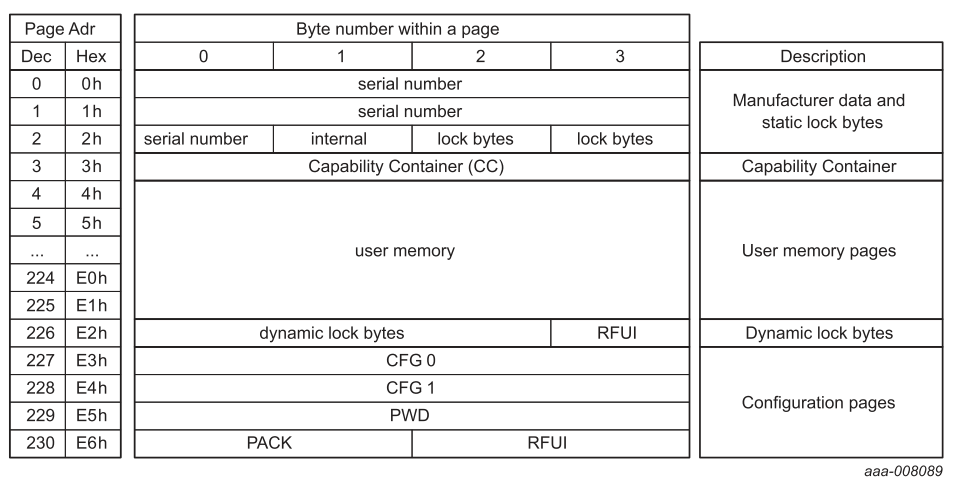
\includegraphics[width=1\textwidth]{material/ntag216-memory}
    \caption{NTAG216 organizacija memorije\cite{NTAG216}}
    \label{fig:ntag_mem}
\end{figure}

\subsection{NDEF \textit{(en. NFC Data Exchange Format)}}
NDEF specifikacija definiše \textbf{format enkapsulacije poruke} za razmjenu informacija između dva NFC uređaja. NDEF je lagan binarni format poruke i može se koristiti za enkapsulaciju jednog ili više aplikacijski-definisanih tereta \textit{(en. payload)} raznih vrsta i veličina unutar jedne NDEF poruke. Svaki teret opisan je od strane tipa, dužine i opcionalnog identifikatora. Identifikatori tipa mogu biti URI, MIME media tipovi, ili NFC-specifični tipovi. NDEF je striktno \textbf{format} poruke i ne poznaje pojam konekcije ili logičkog kola.\cite{NDEF}

\paragraph*{}
Neki od ciljeva koje NDEF nastoji da ispuni:
\begin{itemize}[noitemsep]
    \item enkapsulacija dokumenata i binarnih objekata, slika etc.
    \item enkapsulacija podataka nepoznate dužine, npr. stream-a podataka
    \item agregacija srodnih sadržaja unutar jedne poruke
    \item kompaktna enkapsulacija malih datagrama
\end{itemize}

\subsection{HCE \textit{(en. Host card emulation)}}
HCE je metod emuliranja virtuelnog identifikacijskog modula korisnika, u osnovi to je način zaobilaska hardverskih ograničenja (\textit{en. hack, workaround}) koja onemogućavaju direktan pristup SIM (\textit{en. Subscriber Identification Module}) modulu kod mobilnih telefonskih uređaja\cite{elenkov_2012}, ovakvo rješenje vuče korijene iz ekonomske realnosti sektora mobilnih komunikacija i kartičnog plaćanja, koja se najpreciznije može okarakterisati kao oligopol, naime Google je nastojao integrisati SIM karticu unutar Android operativnog sistema u vidu eSE (\textit{en. embedded Secure Element}) korištenjem već postojeće SIM kartice operatera a u svrhu razvoja Google Wallet rješenja, no to nije odgovaralo operaterima i odbili su suradnju, nakon toga Google iznalazi alternativne načine rješenja problema poput HCE\cite{randomoracle_2014}.

\paragraph*{}
HCE na Android OS radi, kako i naziv govori u CE (\textit{en. Card Emulation}) SLAVE modu, gdje se na svaki BUMP sa NFC čitačem odašilju pripremljeni podaci. Podaci koji se pri tome šalju moraju pratiti standard kartice koju žele emulirati i najčešće se vrši prijenos dokumenta ili datagrama unutar jednog ili više NDEF paketa. Logit koristi pristup prijenosa JSON formatiranog SPIM objekta \texttt{plain/text} unutar jednog NDEF paketa. Radi se o konceptu sa mnoštvom implementacijskih detalja, te zbog sažetosti za više detalja konsultujte oficijelnu dokumentaciju \url{https://developer.android.com/guide/topics/connectivity/nfc/hce}, dok je izvrstan logički prikaz sa primjerima dao Elenkov\cite{Elenkov2015}.

\section{Ostalo}
Dodatno koristi se Android arhitektura za dobavljanje geolokacije\cite{geoa} uz reverzno geokodiranje od strane OpenStreetMap Nominatim projekta\cite{nominatim}. Za potpisivanje i enkripciju korisničkih podataka koristi se RSA\cite{rivest1978method} kriptografija sa 2048 bit ključem. LAPI je Python flask API, kompletan listing koda dostupan je na GitHub u repozitorijima \texttt{koljenovic/logit} i \texttt{koljenovic/logit-node}.